\documentclass[tikz,border=1mm]{standalone}

\usepackage{amsmath}
\usepackage{graphicx}
\renewcommand\familydefault{\sfdefault} 
\usepackage[T1]{fontenc}

\usetikzlibrary{arrows,shapes,calc,math,decorations.fractals,patterns,backgrounds,decorations.markings}
\tikzset{every picture/.style={/utils/exec={\sffamily}}}
\tikzset{point/.style={fill,circle,inner sep=1.5pt}}
\tikzset{vec/.style={-triangle 45,blue,line width=1pt}}
\tikzset{vel/.style={-triangle 45,blue!50!black,line width=1pt}}
\tikzset{acc/.style={-triangle 45,red,line width=1pt}}
\tikzset{myarrow/.style={decoration={markings,mark=at position 1 with {\arrow[scale=3,>=stealth]{>}}},postaction={decorate}}}
\tikzset{dblarrow/.style={latex'-latex'}}
\tikzset{axis/.style={-stealth',line width=1pt}}
\tikzset{mylabel/.style  args={at #1 #2  with #3}{
    postaction={decorate,
    decoration={
      markings,
      mark= at position #1
      with  \node [#2] {#3};
 } } } }

\begin{document}

% % Pendulum
% \begin{tikzpicture}[auto]
%     \draw (0, 0) -- (315:3) node [fill, circle, inner sep=2pt] (1) {};
%     \draw [dashed] (0, 0) -- (0, -3);
%     \draw (315:1) arc (315:270:1);
%     \draw [-triangle 45,shorten <= 2pt] (1) -- ++(0, -1) node [right] {$g$};
%     \draw [latex'-latex'] (45:0.25) -- node {$L$} ++(315:3);
%     \node at (293:0.67) {$\theta$};
%     \draw [-latex', shorten <= 4pt] (1) arc (315:285:3);
% \end{tikzpicture}

% Euler method
% \begin{tikzpicture}
%     \coordinate (0) at (0,1);
%     \coordinate (1) at (3,{0.1*3^2+0.2*3+1});
%     \coordinate (2) at (6,{0.1*6^2+0.2*6+1});
%     \draw [help lines,dashed] (0,0) -- (0) (3,0) -- (1) (6,0) -- (2);
%     \draw [axis] (-1,0) -- ++(8,0) node [below] {$t$};
%     \draw [axis] (-1,0) -- ++(0,6) node [left] {$y$};
%     \draw [domain=-0.5:6.2, smooth, variable=\x, blue,mylabel=at 0.8 above left with {exact solution},line width=1pt] plot ({\x}, {0.1*\x^2+0.2*\x+1});
%     \node [point,red,label=below left:\color{red}$y_n$] (y0) at (0,0.8) {};
%     \node [point,red,label=below right:\color{red}$y_{n+1}$] (y1) at ($(y0)+(3,0.6)+(0,-0.2)$) {};
%     \node [point,red,label=below right:\color{red}$y_{n+2}$] (y2) at ($(y1)+(3,2.4)+(0,-0.2)$) {};
%     \draw [red,line width=1pt] (y0) -- (y1) -- (y2) node [pos=0.5,below right] {numerical solution};
%     \node [below] at (0,0) {$t_n$};
%     \node [below] at (3,0) {$t_{n}+h$};
%     \node [below] at (6,0) {$t_{n}+2h$};
%     \draw [line width=1pt,dashed] ($(0)+(-0.5,-0.1)$) -- ($(0)+(3,0.6)$);
%     \draw [line width=1pt,dashed] ($(1)+(-0.5,-0.4)$) -- ($(1)+(3,2.4)$) node [right] {tangent line};
%     \node [point,blue,label=above:\color{blue}$y(t_n)$] at (0) {};
%     \node [point,blue,label=above left:\color{blue}$y(t_{n}+h)$] at (1) {};
%     \node [point,blue,label=above left:\color{blue}$y(t_{n}+2h)$] at (2) {};
% \end{tikzpicture}


% Graph
% \begin{tikzpicture}
%     \tikzmath{\r=1;}
%     \node [point] at (0:\r) (1) {};
%     \node [point] at (60:\r) (2) {};
%     \node [point] at (120:\r) (3) {};
%     \node [point] at (180:\r) (4) {};
%     \node [point] at (240:\r) (5) {};
%     \node [point] at (300:\r) (6) {};
%     \draw (1) to (2) (1) to (4) (2) to (3) (2) to (5) (5) to (1) (4) to (6);
% \end{tikzpicture}

% Tree
% \begin{tikzpicture}
%     \tikzmath{\r=1;}
%     \node [point] at (0:\r) (1) {};
%     \node [point] at (60:\r) (2) {};
%     \node [point] at (120:\r) (3) {};
%     \node [point] at (180:\r) (4) {};
%     \node [point] at (240:\r) (5) {};
%     \node [point] at (300:\r) (6) {};
%     \draw (1) to (4) (2) to (3) (2) to (5) (5) to (1) (4) to (6);
% \end{tikzpicture}

% Rooted trees
% \begin{tikzpicture}[
%     grow = up,
%     sibling distance=1cm,
%     level distance=1cm]
%     \node [point] {}        
%         child {node [point] {}
%             child {node [point] {}}
%         }
%         child {node [point] {}
%             child {node [point] {}}
%             child {node [point] {}}
%         }
%         child {node [point] {}};
% \end{tikzpicture}

% \begin{tikzpicture}
%     \node [point]{};
%     % \node [point,label=right:\large$\mathbf{f}$]{};
% \end{tikzpicture}

% \begin{tikzpicture}[
%     grow = up,
%     sibling distance=1cm,
%     level distance=1cm]
%     \node [point,label=right:$\mathbf{f}'$] {}
%         child {node [point,label=right:$\mathbf{f}$] {}};
% \end{tikzpicture}

% \begin{tikzpicture}[
%     grow = up,
%     sibling distance=1cm,
%     level distance=1cm]
%     \node [point,label=right:$\mathbf{f}''$] {}
%         child {node [point,label=right:$\mathbf{f}$] {}}
%         child {node [point,label=left:$\mathbf{f}$] {}};
% \end{tikzpicture}

% \begin{tikzpicture}[
%     grow = up,
%     sibling distance=1cm,
%     level distance=1cm]
%     \node [point,label=right:$\mathbf{f}'$] {}
%         child {node [point,label=right:$\mathbf{f}'$] {}
%             child {node [point,label=right:$\mathbf{f}$] {}}
%         };
% \end{tikzpicture}

% Rooted tree example
% \begin{tikzpicture}[
%     grow = up,
%     sibling distance=1cm,
%     level distance=1cm]
%     \node [point,label=right:7] {}        
%         child {node [point,label=right:2] {}
%             child {node [point,label=1] {}}
%         }
%         child {node [point,label=right:3] {}
%             child {node [point,label=1] {}}
%             child {node [point,label=1] {}}
%         }
%         child {node [point,label=left:1] {}};
% \end{tikzpicture}

% \begin{tikzpicture}[
%     grow = up,
%     sibling distance=1cm,
%     level distance=1cm]
%     \node [point,label=right:$i$] {}        
%         child {node [point,label=right:$k$] {}
%             child {node [point] {}}
%         }
%         child {node [point,label=right:$j$] {}
%             child {node [point] {}}
%             child {node [point] {}}
%         }
%         child {node [point] {}};
% \end{tikzpicture}

% Rooted trees up to order 4
% \begin{tikzpicture}
%     \node [point] {};
% \end{tikzpicture}

% \begin{tikzpicture}[
%     grow = up,
%     sibling distance=0.5cm,
%     level distance=0.5cm]
%     \node at (2,0) [point] {}
%         child {node [point] {}};
% \end{tikzpicture}

% \begin{tikzpicture}[
%     grow = up,
%     sibling distance=0.5cm,
%     level distance=0.5cm]
%     \node at (4,0) [point] {}
%         child {node [point] {}}
%         child {node [point] {}};
% \end{tikzpicture}

% \begin{tikzpicture}[
%     grow = up,
%     sibling distance=0.5cm,
%     level distance=0.5cm]
%     \node at (6,0) [point] {}
%         child {node [point] {}
%             child {node [point] {}}
%         };
% \end{tikzpicture}

% \begin{tikzpicture}[
%     grow = up,
%     sibling distance=0.5cm,
%     level distance=0.5cm]
%     \node at (8,0) [point] {}
%         child {node [point] {}}
%         child {node [point] {}}
%         child {node [point] {}};
% \end{tikzpicture}

% \begin{tikzpicture}[
%     grow = up,
%     sibling distance=0.5cm,
%     level distance=0.5cm]
%     \node at (10,0) [point] {}
%         child {node [point] {}
%             child {node [point] {}}
%             child {node [point] {}}
%         };
% \end{tikzpicture}

% \begin{tikzpicture}[
%     grow = up,
%     sibling distance=0.5cm,
%     level distance=0.5cm]
%     \node at (12,0) [point] {}
%         child {node [point] {}
%             child {node [point] {}}
%         }
%         child {node [point] {}};
% \end{tikzpicture}

% \begin{tikzpicture}[
%     grow = up,
%     sibling distance=0.5cm,
%     level distance=0.5cm]
%     \node at (14,0) [point] {}
%         child {node [point] {}
%             child {node [point] {}
%                 child {node [point] {}
%                 }
%             }
%         };
% \end{tikzpicture}

% Rooted trees exercise
% \begin{tikzpicture}[
%     grow = up,
%     level 1/.style={sibling distance=2cm},
%     level 2/.style={sibling distance=0.67cm},
%     level distance=1cm,
%     every node/.style=point]
%     \node {}
%         child {node {}
%             child {node {}}
%             child {node {}
%                 child {node {}}
%                 child {node {}}
%             }
%         }
%         child {node [point] {}
%             child {node {}}
%             child {node {}}
%             child {node {}}
%         };
% \end{tikzpicture}


% Rooted trees exercise (elementary weights and density)
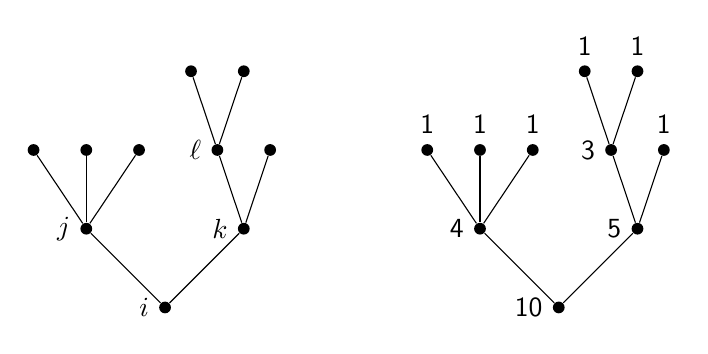
\begin{tikzpicture}[
    grow = up,
    level 1/.style={sibling distance=2cm},
    level 2/.style={sibling distance=0.67cm},
    level distance=1cm,]
    \node [point,label=left:$i$] {}
        child {node [point,label=left:$k$] {}
            child {node [point] {}}
            child {node [point,label=left:$\ell$] {}
                child {node [point] {}}
                child {node [point] {}}
            }
        }
        child {node [point,label=left:$j$] {}
            child {node [point] {}}
            child {node [point] {}}
            child {node [point] {}}
        };
    \node at (5,0) [point,label=left:10] {}
        child {node [point,label=left:5] {}
            child {node [point,label=above:1] {}}
            child {node [point,label=left:3] {}
                child {node [point,label=above:1] {}}
                child {node [point,label=above:1] {}}
            }
        }
        child {node [point,label=left:4] {}
            child {node [point,label=above:1] {}}
            child {node [point,label=above:1] {}}
            child {node [point,label=above:1] {}}
        };
\end{tikzpicture}

% % Interval of absolute stability
% \begin{tikzpicture}
%     \fill [white] (-6, -3) rectangle (4, 3);
%     \draw [fill=blue!20!white,line width=1pt] (-1.5, 0) circle (1.5cm);
%     \draw [-stealth'] (-4, 0) -- (2, 0) node [below] {$\operatorname{Re}(z)$};
%     \draw [-stealth'] (0, -2.5) -- (0, 2.5) node [left] {$\operatorname{Im}(z)$};
%     \draw [latex'-latex', shorten >= 2pt, shorten <= 2pt] (-3, -0.25) -- node [below,text width=2cm,align=center] {stability interval} (0, -0.25);
%     \node at (-4, 2) (1) {stability region};
%     \draw [-latex'] (1) -- ($(-1.5,0)+(135:1.5)$);
%     \node at (-1.5, 0.5) {$|R(z)| < 1$};
%     \node at (1.5, 1.5) {$|R(z)| > 1$};
% \end{tikzpicture}

% Gram-Schmidt
% \begin{tikzpicture}
%     \tikzmath{\a1=15;\a2=60;\l1=5;\l2=4;\ql=1.5;}
%     \draw [vec] (0, 0) -- (\a1:\l1) node [align=center] at (\a1:\l1+0.2) {$\mathbf{a}_1$ \\ $\mathbf{u}_1$};
%     \draw [vec] (0, 0) -- (\a2:\l2) node at (\a2:\l2+0.2) {$\mathbf{a}_2$};
%     \draw [vec,green!50!black] (0,0) -- (\a1+90:{\l2*cos(\a1+90-\a2)}) node [left] {$\mathbf{u}_2$};
%     \draw [vec,black] ($(0,0)$) -- ++(\a1:{\l2*cos(\a2-\a1)}) node [pos=0.75,below,rotate=\a1] (\a1+90:\l2+0.2) {$(\mathbf{a}_2 \cdot \mathbf{q}_1) \mathbf{q}_1$};
%     \draw [vec,red] (0,0) -- (\a1:\ql) node [pos=0.5,below] {$\mathbf{q}_1$};
%     \draw [vec,red] (0,0) -- (\a1+90:\ql) node [pos=0.5,left] {$\mathbf{q}_2$};
%     \draw [vec,black] (\a2:\l2) -- ++(\a1+180:{\l2*cos(\a2-\a1)}) node [pos=0.5,rotate=\a1,above] {$-(\mathbf{a}_2 \cdot \mathbf{q}_1) \mathbf{q}_1$};
%     \draw [help lines,dashed] (\a2:\l2) -- (\a1:{\l2*cos(\a2-\a1)});
% \end{tikzpicture}

% Householder
% \begin{tikzpicture}
%     \tikzmath{\a1=0;\a2=45;\l1=4;}
%     \draw [vec] (0, 0) -- (\a2:\l1) node [above right] {$\mathbf{x}$};
%     \draw [vec,red] (0, 0) -- (\a1:\l1) node [pos=0.67,below] {$\|\mathbf{x}\|\mathbf{e}_1$};
%     \draw [dashed] (0, 0) -- (0.5*\a2:5);
%     \draw [vec,green!75!black] (\a1:\l1) -- (\a2:\l1) node [pos=0.67,above right] {$\mathbf{u}$};
%     \draw [vec,black] (0, 0) -- (\a1:1.5) node [below,pos=0.5] {$\mathbf{e}_1$};
%     \draw [vec,black] (\a1:\l1) -- ($(\a1:\l1)!0.4!(\a2:\l1)$) node [pos=0.5,right] {$\mathbf{v}$};
%     \draw [-latex',bend left,shorten >= 4pt, shorten <= 4pt] (\a2:0.5*\l1) to (\a1:0.5*\l1);
% \end{tikzpicture} 

% \begin{tikzpicture}
%     \tikzmath{\a1=0;\a2=45;\l1=4;}
%     \draw [vec] (0, 0) -- (\a2:\l1) node [above right] {$\mathbf{x}$};
%     \draw [vec,red] (0, 0) -- (\a1:-\l1) node [pos=0.67,below] {$-\|\mathbf{x}\|\mathbf{e}_1$};
%     \draw [dashed] (0, 0) -- (0.5*\a2+90:4);
%     \draw [vec,green!75!black] (\a1:-\l1) -- (\a2:\l1) node [pos=0.8,above left] {$\mathbf{u}$};
%     \draw [vec,black] (0, 0) -- (\a1:1.5) node [below,pos=0.5] {$\mathbf{e}_1$};
%     \draw [vec,black] (\a1:-\l1) -- ($(\a1:-\l1)!0.2!(\a2:\l1)$) node [pos=0.5,above left] {$\mathbf{v}$};
%     \draw [-latex',bend right,shorten >= 4pt, shorten <= 4pt] (\a2:0.33*\l1) to (\a1:-0.33*\l1);
% \end{tikzpicture}

% SOR method
% \begin{tikzpicture}
%     \draw [-stealth'] (0, 0) -- (6, 0) node [right] {iterations};
%     \draw [-stealth'] (0, 0) -- (0, 4) node [above] {$x_i$};
%     \draw [dashed] (0, 2) -- (6, 2) node [above] {exact solution};
%     \node [draw, blue, fill=blue, circle, inner sep=1pt] at (0, 0) (0) {};
%     \node [draw, blue, fill=blue, circle, inner sep=1pt] at (1, 0.8) (1) {};
%     \node [draw, blue, fill=blue, circle, inner sep=1pt] at (2, 1.28) (2) {};
%     \node [draw, blue, fill=blue, circle, inner sep=1pt] at (3, 1.57) (3) {};
%     \node [draw, blue, fill=blue, circle, inner sep=1pt] at (4, 1.74) (4) {};
%     \node [draw, blue, fill=blue, circle, inner sep=1pt] at (5, 1.84) (5) {};
%     \draw [blue] (0) -- (1) -- (2) -- (3) -- (4) -- (5);
%     \draw [-latex', shorten >= 2pt] (2.5, 1) node [anchor=north west] {Gauss-Seidel} -- (2);
%     \node [draw, red, fill=red, circle, inner sep=1pt] at (1, 1.3) (1) {};
%     \node [draw, red, fill=red, circle, inner sep=1pt] at (2, 1.7) (2) {};
%     \node [draw, red, fill=red, circle, inner sep=1pt] at (3, 1.82) (3) {};
%     \node [draw, red, fill=red, circle, inner sep=1pt] at (4, 1.91) (4) {};
%     \node [draw, red, fill=red, circle, inner sep=1pt] at (5, 1.96) (5) {};
%     \draw [red] (0) -- (1) -- (2) -- (3) -- (4) -- (5);
%     \draw [-latex', shorten >= 2pt] (2, 2.5) node [anchor=south] {over relaxed solution} -- (2);
% \end{tikzpicture}

% \begin{tikzpicture}
%     \draw [-stealth'] (0, 0) -- (6, 0) node [right] {iterations};
%     \draw [-stealth'] (0, 0) -- (0, 4) node [above] {$x_i$};
%     \draw [dashed] (0, 2) -- (6, 2) node [below] {exact solution};
%     \node [draw, blue, fill=blue, circle, inner sep=1pt] at (0, 0) (0) {};
%     \node [draw, blue, fill=blue, circle, inner sep=1pt] at (1, 3.2) (1) {};
%     \node [draw, blue, fill=blue, circle, inner sep=1pt] at (2, 1.28) (2) {};
%     \node [draw, blue, fill=blue, circle, inner sep=1pt] at (3, 2.43) (3) {};
%     \node [draw, blue, fill=blue, circle, inner sep=1pt] at (4, 1.74) (4) {};
%     \node [draw, blue, fill=blue, circle, inner sep=1pt] at (5, 2.16) (5) {};
%     \draw [blue] (0) -- (1) -- (2) -- (3) -- (4) -- (5);
%     \draw [-latex', shorten >= 2pt] (2.5, 1) node [anchor=north west] {Gauss-Seidel} -- (2);
%     \node [draw, red, fill=red, circle, inner sep=1pt] at (1, 2.6) (1) {};
%     \node [draw, red, fill=red, circle, inner sep=1pt] at (2, 1.64) (2) {};
%     \node [draw, red, fill=red, circle, inner sep=1pt] at (3, 2.22) (3) {};
%     \node [draw, red, fill=red, circle, inner sep=1pt] at (4, 1.92) (4) {};
%     \node [draw, red, fill=red, circle, inner sep=1pt] at (5, 2.08) (5) {};
%     \draw [red] (0) -- (1) -- (2) -- (3) -- (4) -- (5);
%     \draw [-latex', shorten >= 2pt] (1.5, 3) node [anchor=south west] {under relaxed solution} -- (1);
% \end{tikzpicture}

\end{document}